Fishing grounds in WPP 714+715 are combined for analysis as they are ecologically closely connected and the dynamics of the fleet also covers these 2 WPP as a single fishing area. The presented Spot trace data from the WPP 714 and 715 shows great mobility of the medium-scale snapper fishing boats, making trips to fishing grounds that are up to 1,000 kilometers away from home ports. Not only are these fleets highly mobile in terms of their trips from home port, they are also flexible in changing their base of operations from one port to another, changing from landing at home port to offloading on transport vessels in remote ports or offloading for air cargo at yet other places. Decision making on movements by boat owners can be based on fisheries technical issues such as catch rates or weather, but also on administrative issues like licensing or enforcement of rules against under-marking in Gross Tonnage. Most recently we are observing movement of staging ports but also of processing capacity to remote areas in the east such as Ternate and the island of Penambulai, East of the Aru Islands. Fish is landed there and moved onto transport vessels bound for processing plants elsewhere in the country.

Small scale fleets from the Banggai and Sula Island as well as from mainland Sulawesi and other locations, feed into the same supply lines as the medium scale fishery, via a network of small local traders that eventually aggregates larger volumes for sale to processing companies. For example a major snapper processor based in Luwuk, Central Sulawsi, receives part of its raw product from the supply network around the local islands. But this company is also receiving large transports from Kema in North Sulawesi, which is the base of a medium scale deep water snapper drop line fishery. That fishery currently lands most of its catches in Kema but operates throughout and beyond the waters of WPP 715 and 714. Therefore the fish that is processed in Luwuk comes from a number of different fleets that operate throughout the waters of WPP 715 and 714 and beyond. At the same time, medium scale fishing boats originating from ports well outside this area also operate regularly (but not constantly) in WPP 714 and 715. For the purpose of this report, all fishing trips, recorded within WPP 714 and / or 715, small and / or medium scale, were included in the analysis for WPP 714+715. This includes fishing trips originating from outside the WPPs, for example from Probolinggo, Bali or Kupang.

Potential IUU issues include the under marking of medium scale vessels to below 30GT, the licensing of the various fleets for various WPP and the operation of deep slope snapper fishers from remote ports at deep water sites inside Marine Protected Areas throughout this region. Especially the fisheries activity by Kema boats in the Raja Ampat area and around Kaimana, in the recently developed "Bird's Head MPA Network", needs to be discussed with fishing boat captains and boat owners to prevent issues of supply line "pollution" with IUU fish from thee protected areas.

\begin{center}
\graphicspath{{/root/R-project/IFishSnapperWPP714_715/Images/}}
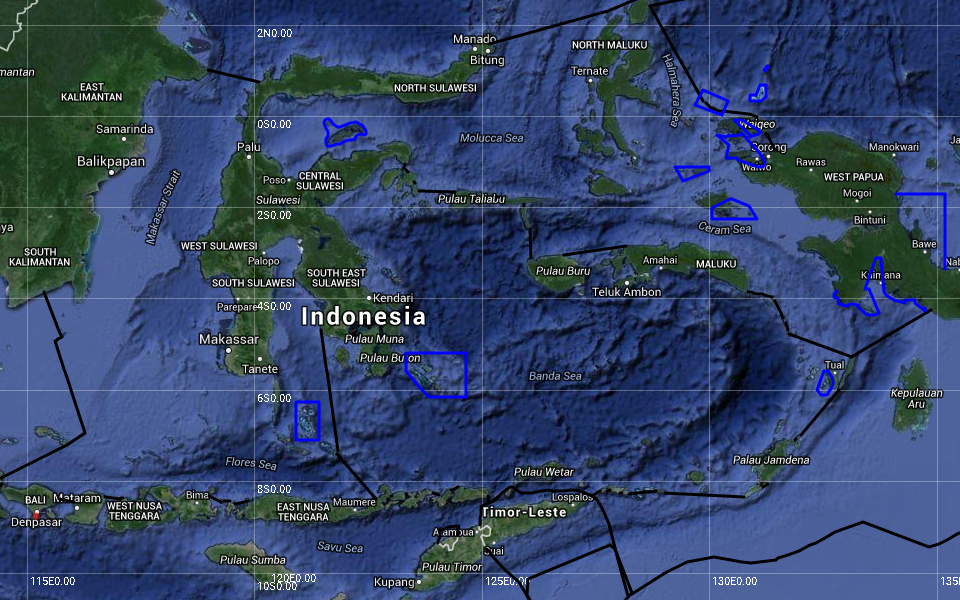
\includegraphics[width=15cm]{AreaC-Satellite.jpg}

Figure 8. Bathymetric map of WPPs 714 \& 715, with important Marine Protected Areas. Black lines are WPP boundaries, blue lines are MPA boundaries.
\end{center}

\begin{center}
\graphicspath{{/root/R-project/IFishSnapperWPP714_715/Images/}}
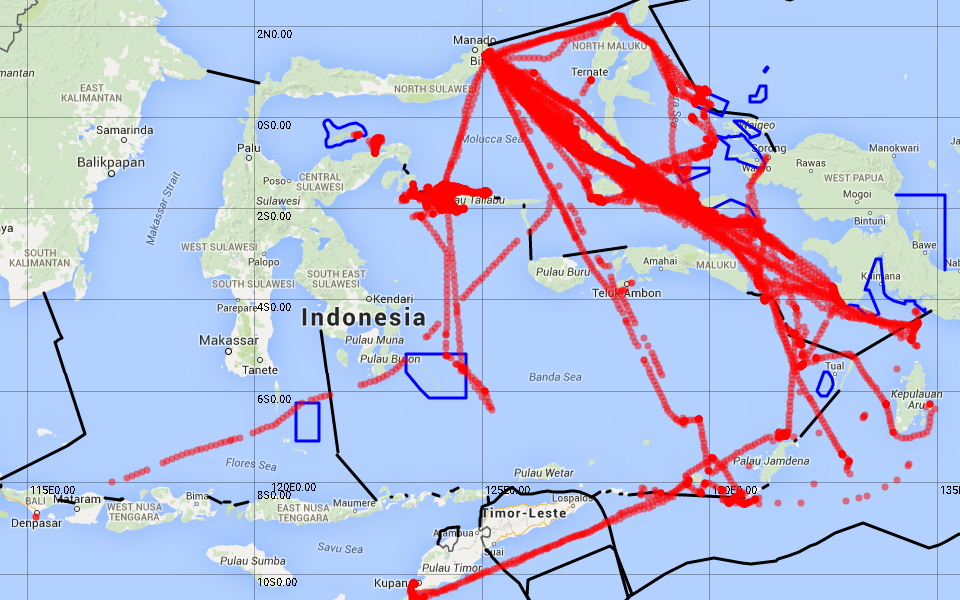
\includegraphics[width=15cm]{SpotTrace-AreaC.jpg}

Figure 9. Map with aggregated Spot Trace data from snapper fishing vessels operating in WPP 714 and 715. Red dots in a line represent the tracks of travelling fishing vessels, whereas dots in a cluster represent fishing activity.
\end{center}

\begin{center}
\graphicspath{{/root/R-project/IFishSnapperWPP714_715/Images/}}
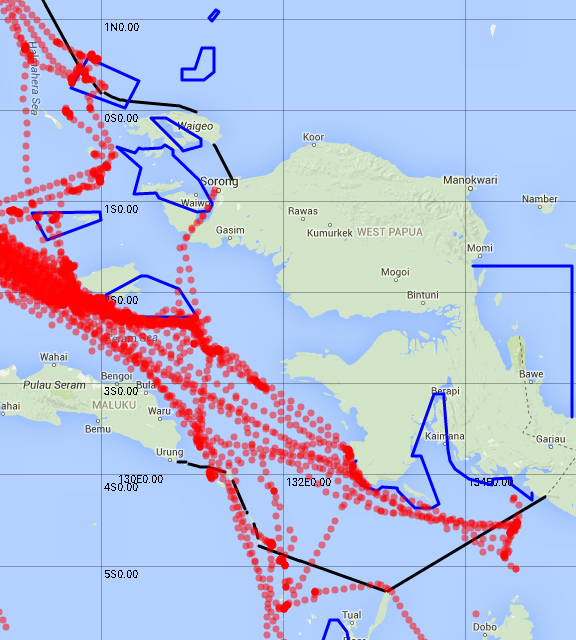
\includegraphics[width=15cm]{SpotTrace-AreaC-BirdHead.jpg}

Figure 10. Map with aggregated Spot Trace data from snapper fishing vessels operating around the Bird�s Head of West Papua in WPP 715. Red dots in a line represent the tracks of travelling fishing vessels, whereas dots in a cluster represent fishing activity. The black line represents the boundary of WPP 715 and the blue lines represent the boundaries of the Bird�s Head MPA network including the Raja Ampat and Kaimana MPAs.
\end{center}

\begin{center}
\graphicspath{{/root/R-project/IFishSnapperWPP714_715/Images/}}
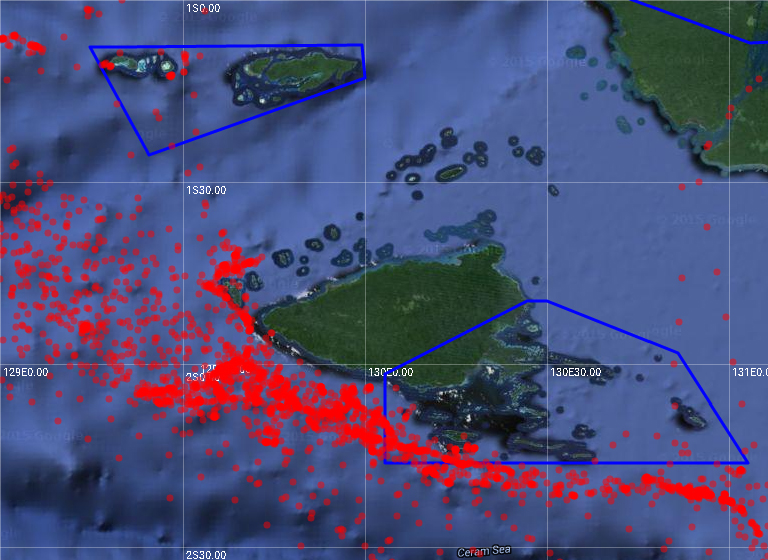
\includegraphics[width=15cm]{SpotTrace-AreaC-Misool-Satellite.jpg}

\graphicspath{{/root/R-project/IFishSnapperWPP714_715/Images/}}
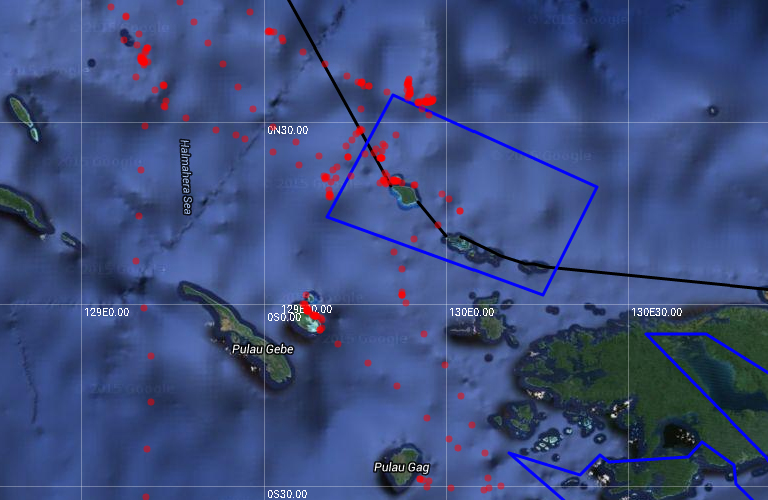
\includegraphics[width=15cm]{SpotTrace-AreaC-Kawe-Satellite.jpg}

Figure 11. Fishing activity by snapper boats (clusters of red dots) in and around Raja Ampat MPAs at Misool \& Kofiau (top) and Sayang \& Wayag (bottom) island groups.
\end{center}

\begin{center}
\graphicspath{{/root/R-project/IFishSnapperWPP714_715/Images/}}
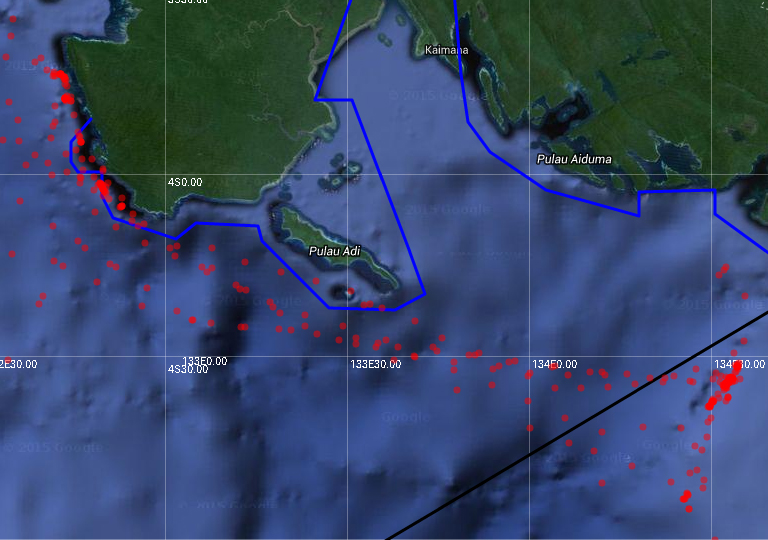
\includegraphics[width=15cm]{SpotTrace-AreaC-Kaimana-Satellite.jpg}

\graphicspath{{/root/R-project/IFishSnapperWPP714_715/Images/}}
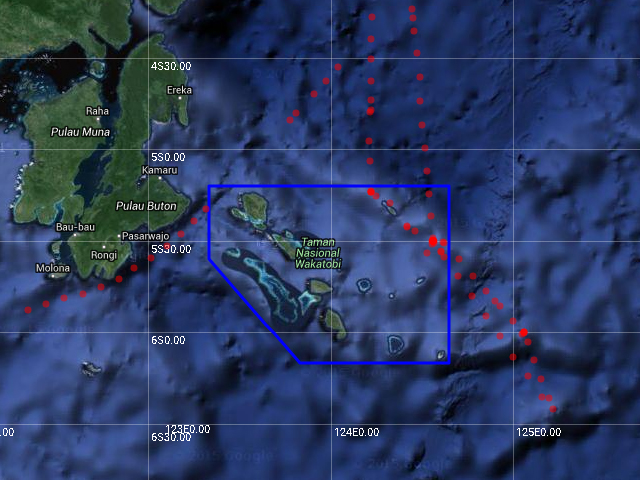
\includegraphics[width=15cm]{SpotTrace-AreaC-Wakatobi-Satellite.jpg}

Figure 12. Fishing activity (clusters of red dots) from snapper boats in and around MPAs at Kaimana (top) and Wakatobi National Park (bottom) in WPP 715 and WPP 714.
\end{center}

\begin{center}
\graphicspath{{/root/R-project/IFishSnapperWPP714_715/Images/}}
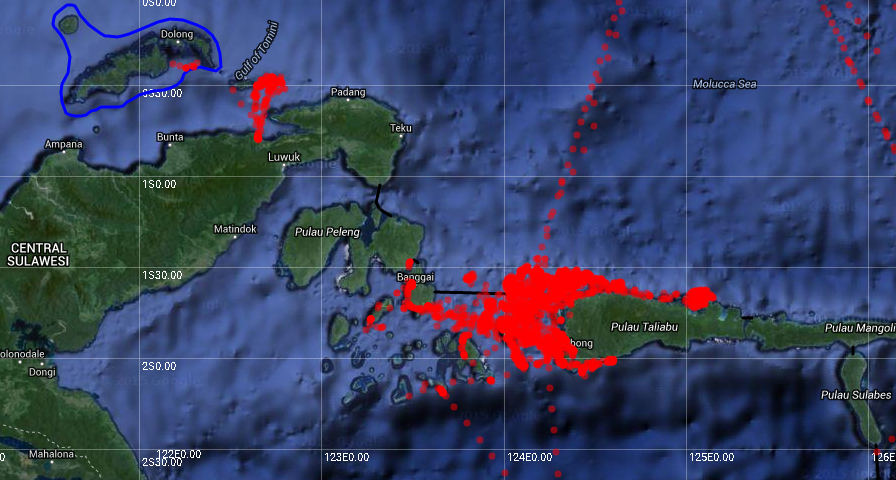
\includegraphics[width=15cm]{SpotTrace-AreaC-Luwuk-Satellite.jpg}

Figure 13. WPP 714 and 715 fishing activity (clusters of red dots) from small scale snapper boats making short trips near home islands and supplying (via traders) a processor based in Luwuk, Central Sulawesi. Activity of small boats is dense around the Sula Islands, with less activity in the Banggai Islands and in Tomini Bay, including the Togean Islands National Park.
\end{center}